\subsection{Bestimmung der Verdampungswärme bei kleinem Druck}

\begin{figure}[h!]
	\centering
	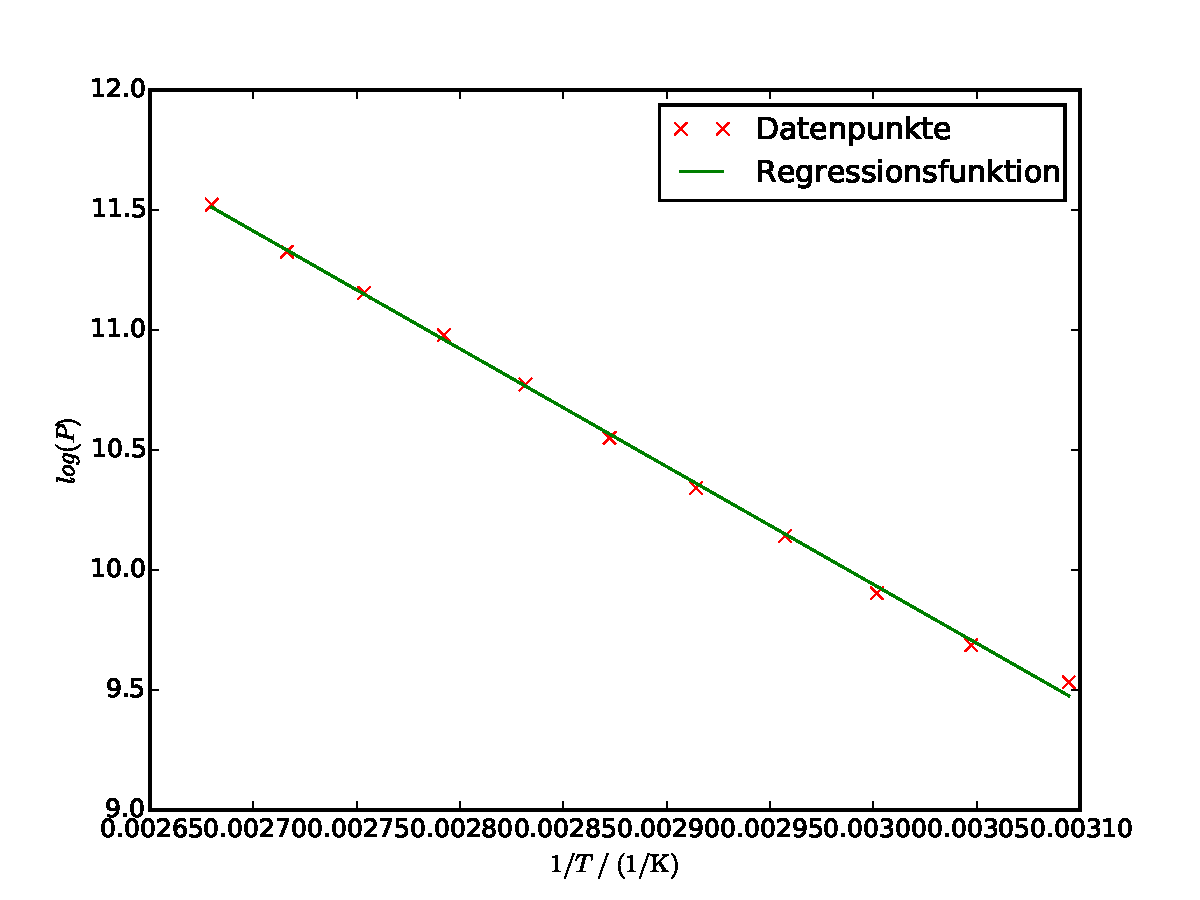
\includegraphics[width=0.95\textwidth]{L_kleiner_Druck.pdf}
	\caption{Logarithmus des Dampfdruckes gegen die reziproke absolute Temperatur}
	\label{fig:L_kleiner_Druck}
\end{figure}

\subsection{Temperaturabhängigkeit der Verdampfungswärme bei hohem Druck}

\begin{figure}[h!]
	\centering
	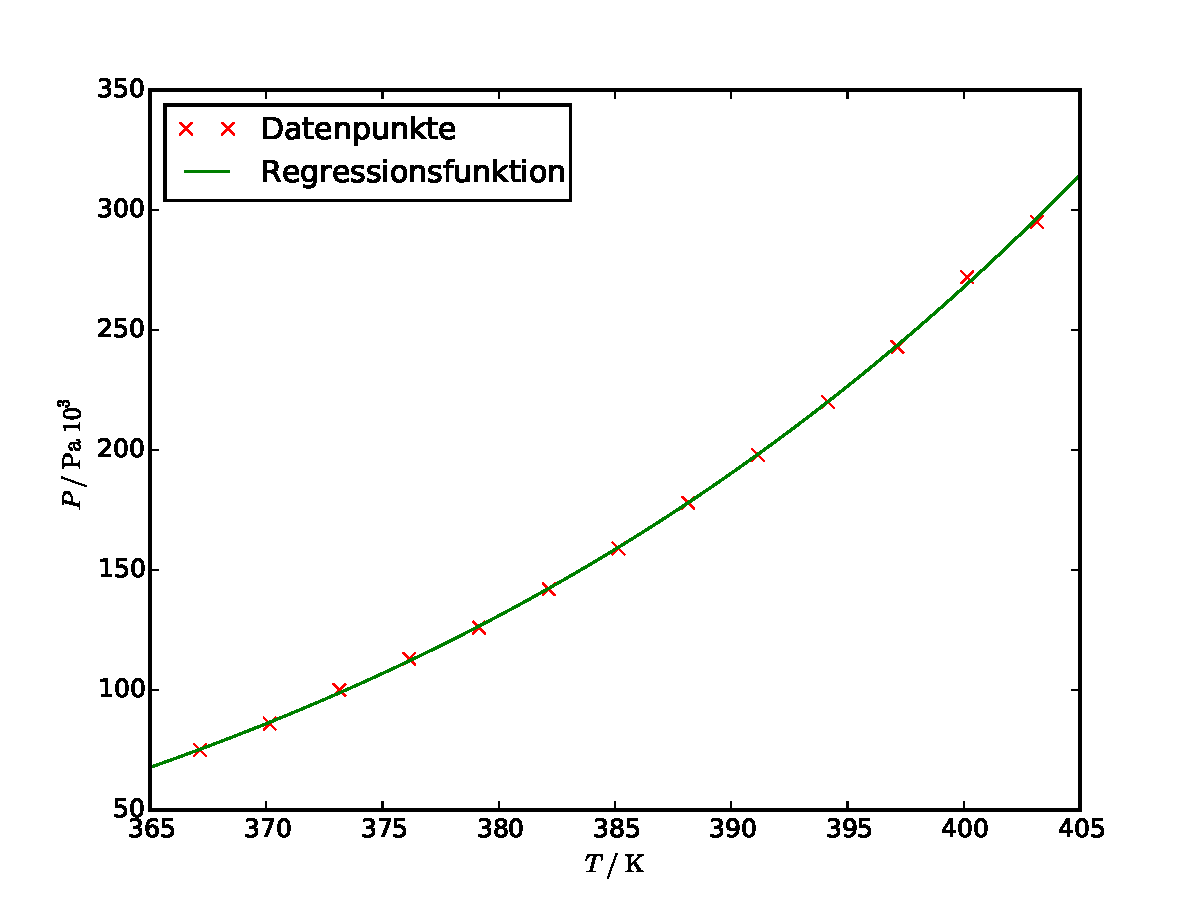
\includegraphics[width=0.95\textwidth]{Regerssionspolynom_P(t).pdf}
	\caption{Regressionspolynom dritten Grades des Druckes über die Temperatur}
	\label{fig:Regerssionspolynom_P(t)}
\end{figure}
\\
\begin{figure}[h!]
	\centering
	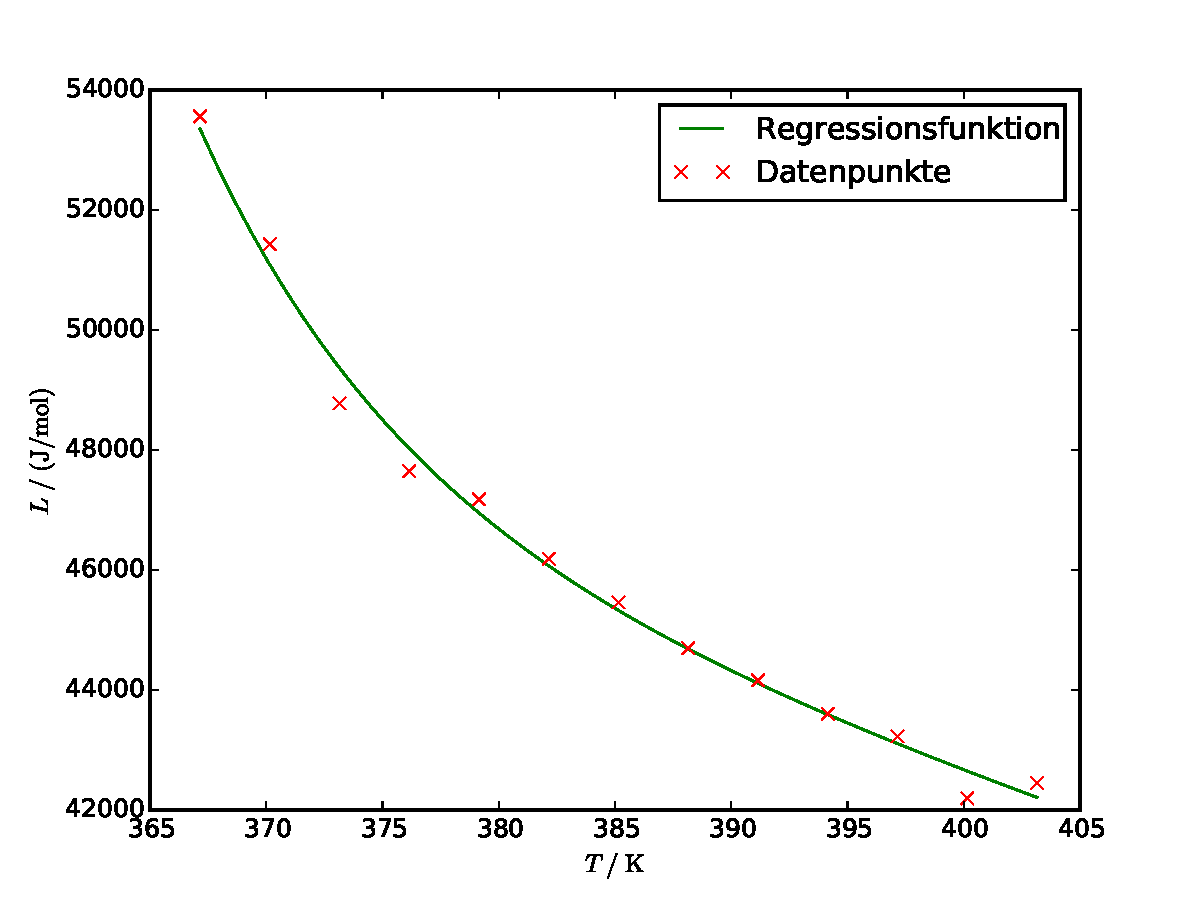
\includegraphics[width=0.95\textwidth]{L_groser_druck_temperaturabhangig.pdf}
	\caption{Verdampfungswärme in Abhängigkeit der Temperatur}
	\label{fig:L_groser_druck_temperaturabhangig}
\end{figure}



